% Setup -------------------------------

\documentclass[a4paper]{report}
\usepackage[a4paper, total={6in, 10in}]{geometry}
\setcounter{secnumdepth}{3}
\setcounter{tocdepth}{3}

\usepackage{hyperref}
\usepackage{indentfirst}

\usepackage{fancyvrb}
\usepackage{xcolor}

\usepackage{graphicx}

\usepackage{float}

% Encoding
%--------------------------------------
\usepackage[T1]{fontenc}
\usepackage[utf8]{inputenc}
%--------------------------------------

% Portuguese-specific commands
%--------------------------------------
\usepackage[portuguese]{babel}
%--------------------------------------

% Hyphenation rules
%--------------------------------------
\usepackage{hyphenat}
%--------------------------------------

% Capa do relatório

\title{
	Gestão de Grandes Conjuntos de Dados
	\\ \Large{\textbf{1º Trabalho Prático}}
	\\ -
	\\ Mestrado em Engenharia Informática
	\\ Universidade do Minho
}
\author{
	\begin{tabular}{ll}
		\textbf{Grupo nº 8}
		\\
		\hline
		PG41080 & João Ribeiro Imperadeiro
        \\
		PG41081 & José Alberto Martins Boticas
		\\
        PG41091 & Nelson José Dias Teixeira
        \\
        PG41851 & Rui Miguel da Costa Meira
	\end{tabular}
}

\date{\today}

\begin{document}

\begin{titlepage}
    \maketitle
\end{titlepage}

% Índice

\tableofcontents
\listoffigures

% Introdução

\chapter{Introdução} \label{ch:Introduction}
\large {
	Na primeira parte deste trabalho prático é requerida a concretização e avaliação experimental de tarefas de armazenamento e processamento de dados utilizando as ferramentas computacionais \textit{Hadoop HDFS}, \textit{HBase} e, ainda, o paradigma \textit{MapReduce}. 
	Por forma a realizar estas tarefas, os dados a utilizar para tal efeito correspondem ao conjunto de dados público do \textit{IMDB}, que se encontram disponíveis em: 
	\begin{center}
		\textit{\url{https://www.imdb.com/interfaces/}}
	\end{center}

	Ao longo deste documento vão também ser expostos todos os passos tomados durante a implementação das tarefas pedidas neste projeto, incluindo as decisões tomadas pelos elementos deste grupo a nível de algoritmos e parâmetros de configuração.
	Para além disso são ainda apresentadas todas as instruções que permitem executar e utilizar corretamente os programas desenvolvidos.
	Por fim, na fase final deste manuscrito, são exibidos os objetivos atingidos após a realização das tarefas propostas.

	De salientar ainda que durante os capítulos que se seguem são identificadas algumas alternativas para concretizar as tarefas indicadas neste trabalho prático.
}

\chapter{Implementação} \label{ch:Implementation}
\large {
	Tal como foi enunciado anteriormente, neste projeto é globalmente solicitada a elaboração de duas tarefas. Apresentam-se de seguida as mesmas:
	\begin{enumerate}
		\item Carregar os dados do ficheiro \textit{"title.basics.tsv.gz"} para uma tabela \textit{HBase};
		\item Utilizando a tabela \textit{HBase} do ponto acima e os restantes ficheiros presentes no \textit{dataset} mencionado no capítulo anterior, computar os dados necessários para apresentar para cada ator uma página. Esta última deve conter:
		\begin{itemize}
			\item nome, datas de nascimento e morte;
			\item número total de filmes em que participou como ator;
			\item títulos dos três filmes com melhor cotação em que participou.
		\end{itemize}
		Estes dados devem ser armazenados numa tabela \textit{HBase}.
	\end{enumerate}
	
	Nas próximas secções são evidenciadas as implementações para cada uma destas tarefas bem como algumas sugestões alternativas que poderiam ser tomadas em consideração.
	\section{1ª Tarefa} \label{sec:Task1}
		Após descarregar o ficheiro \textit{"title.basics.tsv.gz"} presente na hiperligação do capítulo anterior, os elementos que compõem este grupo optaram por converter o mesmo no formato \textit{.tsv}. 
		A tomada desta decisão deve-se ao facto deste último permitir a partição de dados (isto é, potencia o \textbf{paralelismo}), ao contrário do formato \textit{.gz} (\textit{gzip}), e, ainda, ser mais rápido e eficiente no processo de descompressão quando comparado com o formato \textit{.bz2} (\textit{bzip2}).
		Mostra-se na seguinte figura a instrução associada à descompressão do ficheiro \textit{"title.basics.tsv.gz"}:
		\begin{figure}[H]
			{
				\color{teal}
				\begin{verbatim}
                            gzip -d title.basics.tsv.gz
				\end{verbatim}
			}
			\caption{1ª Tarefa - Conversão do ficheiro \textit{"title.basics.tsv.gz"} para o formato \textit{.gz} (\textit{gzip})}
            \label{fig:1}
		\end{figure}

		Antes de observar os passos relativos à realização desta tarefa, passos esses que se encontram explicitamente indicados nos próximos subcapítulos, é importante salientar que a execução das soluções elaboradas nas secções \hyperref[subsec:Task1-1]{2.1.1} e \hyperref[subsec:Task1-3]{2.1.3} são efetuadas com recurso a um ficheiro denominado por \textit{Dockerfile}.
		De forma a entender melhor a configuração do mesmo, revela-se a seguir o seu conteúdo:
		\begin{figure}[H]
			{
				\color{teal}
				\begin{verbatim}
					   FROM bde2020/hadoop-base
					   COPY target/TP1-1.0-SNAPSHOT.jar /
					   ENTRYPOINT ["hadoop", "jar", "/TP1-1.0-SNAPSHOT.jar", "ClassName"]
				\end{verbatim}
			}
            \caption{1ª Tarefa - \textit{Dockerfile}}
            \label{fig:2}
        \end{figure}
        
        Após esta observação, indica-se ainda as opções adotadas para a execução do ficheiro \textit{Dockerfile} com o intuito de garantir uma execução válida das soluções implementadas:
		\begin{figure}[H]
			{
				\color{teal}
				\begin{verbatim}
					   --network docker-hbase_default
					   --env-file ../docker-hbase/hadoop.env
					   --env-file ../docker-hbase/hbase-distributed-local.env
				\end{verbatim}
			}
			\caption{1ª Tarefa - \textit{Dockerfile} - Opções de execução}
			\label{fig:3}
        \end{figure}
		
		\subsection{Criação da tabela \textit{HBase}} \label{subsec:Task1-1}
		De forma a criar a tabela \textit{HBase} intrínseca a esta tarefa, foi implementada uma classe \textit{Java}, \textbf{\textit{CreateTableMovies}}, que, após conectar-se com a base de dados não relacional \textit{HBase}, trata da sua criação e configuração.
		Durante esse processo, é produzida apenas uma família de colunas, intitulada por \textbf{\textit{details}}, onde será armazenada toda a informação associada aos dados do ficheiro \textit{"title.basics.tsv.gz"}.

		De notar também que atribuiu-se o nome \textbf{\textit{movies}} à tabela gerada, tal como o nome da classe \textit{Java} transparece.

		Foi também criada uma classe \textit{Java} adicional, \textbf{\textit{DeleteTableMovies}}, que trata de eliminar a tabela descrita anteriormente.
		Esta foi desenvolvida com o intuito de remover a tabela em causa caso esta deixe se ser necessária no futuro.
        
        Apresenta-se de seguida o modelo da tabela \textit{HBase} pretendido para a concretização desta tarefa:
        \begin{figure}[H]
            \centering
            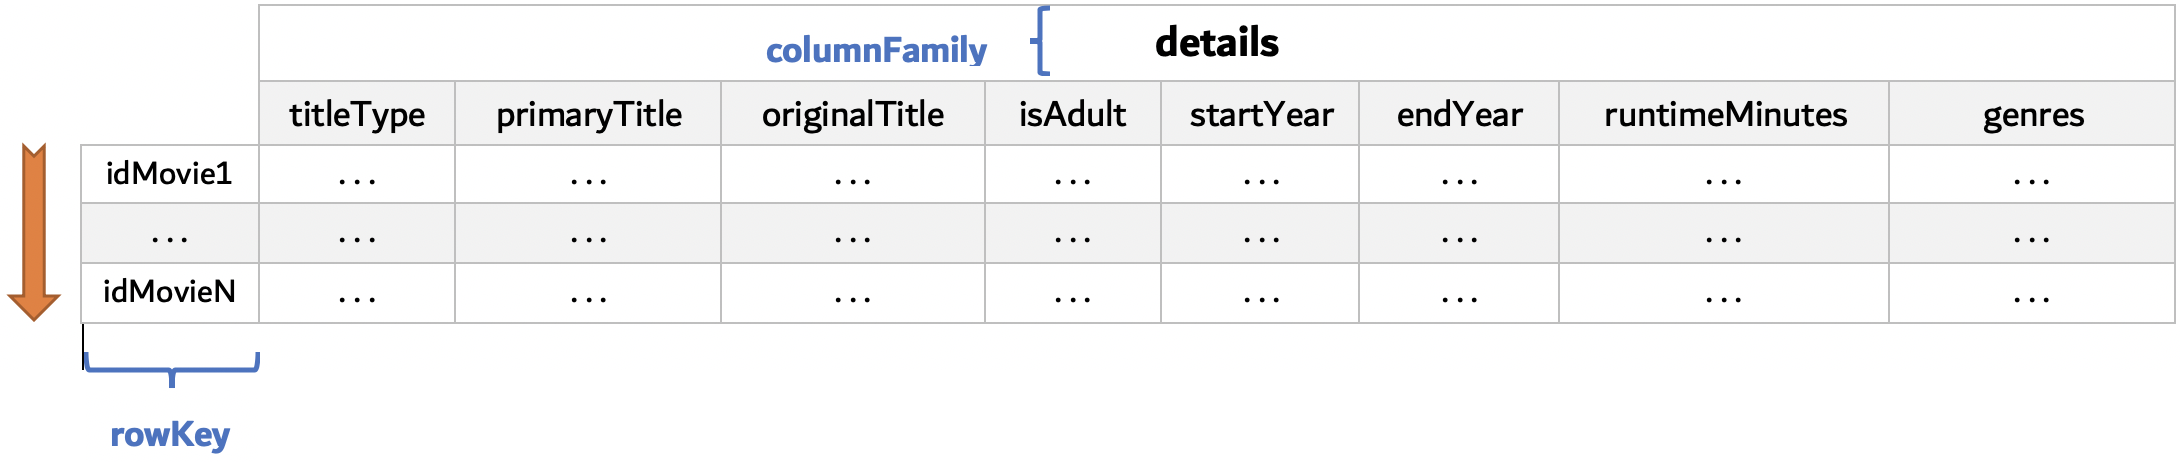
\includegraphics[width=1.0\textwidth]{Imagens/Tabela Hbase.png}
            \caption{1ª Tarefa - Modelo da tabela \textit{HBase "movies"}}
            \label{fig:4}
        \end{figure}

			\subsubsection{Alternativa}
			Uma possibilidade válida para realizar todo o processo associado à criação da tabela requerida seria utilizar a \textit{HBase shell} de forma direta.
			Exibe-se de seguida as respetivas instruções:
			\begin{figure}[H]
				{
					\color{teal}
					\begin{verbatim}
					   docker run -it
					              --network docker-hbase_default
					              --env-file docker-hbase/hbase-distributed-local.env
					              bde2020/hbase-base hbase shell
					\end{verbatim}
				}
				\caption{1ª Tarefa : Alternativa - Acesso à \textit{HBase shell}}
				\label{fig:5}
			\end{figure}

			\begin{figure}[H]
				{
					\color{teal}
					\begin{Verbatim}[commandchars=\\\{\}]
                  \textcolor{orange}{hbase(main):001:0>} create "movies", "details"
					\end{Verbatim}
				}
				\caption{1ª Tarefa : Alternativa - Criação da tabela \textit{HBase "movies"}}
				\label{fig:6}
			\end{figure}
			
			Quanto à remoção da mesma tabela, à semelhança do procedimento tomado para a sua criação, adota-se a estratégia de usufruir explicitamente o mecanismo disponibilizado pela \textit{HBase shell}:
			\begin{figure}[H]
				{
					\color{teal}
					\begin{Verbatim}[commandchars=\\\{\}]
                        \textcolor{orange}{hbase(main):001:0>} disable "movies"
                        \textcolor{orange}{hbase(main):002:0>} drop "movies"
					\end{Verbatim}
				}
				\caption{1ª Tarefa : Alternativa - Remoção da tabela \textit{HBase "movies"}}
				\label{fig:7}
			\end{figure}

		\subsection{Transferência do ficheiro para a plataforma \textit{Hadoop HDFS}} \label{subsec:Task1-2}
		De maneira a proceder ao carregamento do ficheiro \textit{"title.basics.tsv"} para a plataforma \textit{Hadoop HDFS} existem duas possibilidades.
		Antes de exibir estas últimas alternativas, foi criada uma pasta na plataforma \textit{Hadoop HDFS}, denominada por \textit{data}, onde serão colocados todos os ficheiros de \textit{input} necessários.
		Exibe-se de seguida a instrução para tal efeito:
		\begin{figure}[H]
			{
				\color{teal}
				\begin{verbatim}
					   docker run --network docker-hbase_default
					              --env-file docker-hbase/hadoop.env
					              bde2020/hadoop-base hdfs dfs -mkdir /data
				\end{verbatim}
			}
			\caption{1ª Tarefa - Criação da pasta \texttt{data} na plataforma \textit{Hadoop HDFS}}
            \label{fig:8}
		\end{figure}

		Após a exposição deste comando, destacam-se nos próximos subcapítulos as duas alternativas mencionadas acima.

			\subsubsection{1ª Alternativa}
			Nesta possibilidade evidencia-se o campo \texttt{source} que corresponde à diretoria da pasta que contém o ficheiro \textit{"title.basics.tsv"}.
			Dito isto, apresenta-se agora a primeira alternativa:
			\begin{figure}[H]
				{
					\color{teal}
					\begin{verbatim}
					   docker run --network docker-hbase_default
					              --env-file docker-hbase/hadoop.env
					              --mount type=bind,source="/path/to/local/folder/data",target=/data
					              bde2020/hadoop-base hdfs dfs -put /data/title.basics.tsv /data
					\end{verbatim}
				}
				\caption{1ª Tarefa : 1ª Alternativa - Transferência do ficheiro \textit{"title.basics.tsv"} para a plataforma \textit{Hadoop HDFS}}
				\label{fig:9}
			\end{figure}

			\subsubsection{2ª Alternativa}
			Esta opção corresponde ao modo interativo de execução disponibilizado pela instrução \textit{docker run}.
			Uma vez feita esta observação, expõe-se a seguir a segunda alternativa:
			\begin{figure}[H]
				{
					\color{teal}
					\begin{verbatim}
					   docker run -it
					              --network docker-hbase_default
					              --env-file docker-hbase/hadoop.env
					              bde2020/hadoop-base bash

					   curl https://datasets.imdbws.com/title.basics.tsv.gz | gunzip |
					   hdfs dfs -put - hdfs://namenode:9000/data/title.basics.tsv
					\end{verbatim}
				}
				\caption{1ª Tarefa : 2ª Alternativa - Transferência do ficheiro \textit{"title.basics.tsv"} para a plataforma \textit{Hadoop HDFS}}
				\label{fig:10}
			\end{figure}

		\subsection{População da tabela \textit{HBase}} \label{subsec:Task1-3}
		Quanto à população da tabela criada previamente foi igualmente implementada uma classe \textit{Java} para o efeito, designada por \textbf{\textit{PopulateTableMovies}}.
		Esta classe incorpora uma tarefa assente no paradigma \textit{MapReduce}, onde é apenas elaborada a fase de \textit{map}.
		Nessa mesma etapa é processada cada linha do ficheiro de \textit{input} presente na plataforma \textit{Hadoop HDFS} e, quando o tratamento estiver concluído, o resultado obtido é colocado na tabela \textit{movies}.

	\section{2ª Tarefa} \label{sec:Task2}
	Tal como foi descrito no início do 2º capítulo deste documento, esta tarefa é composta por 3 alíneas distintas. Como tal é preciso tomar abordagens diferentes de forma a obter resultados corretos para cada uma das mesmas. 
	Após uma leitura cuidadosa sobre o que é pedido em cada uma destas subtarefas, os elementos deste grupo notaram que iria ser necessário recolher 3 dos ficheiros que fazem parte do \textit{dataset IMDB} para extrair os resultados pretendidos.
	Apresenta-se de seguida os 3 ficheiros escolhidos:
	\begin{itemize}
		\item \textit{"title.basics.tsv"}: informação detalhada dos filmes, nomeadamente o ano de começo, géneros, entre outros;
		\item \textit{"title.principals.tsv"}: conjunto de dados relativos aos atores que integram um determinado filme;
		\item \textit{"title.ratings.tsv"}: informação associada à classificação e votação dos filmes presentes na plataforma \textit{IMDB}.
	\end{itemize}
	
	Tal como se pode observar na listagem acima, o formato utilizado para estes ficheiros é o formato \textit{.tsv}. A escolha desta extensão em detrimento de outras é exatamente a mesma que se encontra no início do subcapítulo relativo à \hyperref[sec:Task1]{1ª tarefa}.
		
		\subsection{Criação da tabela \textit{HBase}} \label{subsec:Task2-1}

		\subsection{Transferência de ficheiros para a plataforma \textit{Hadoop HDFS}} \label{subsec:Task2-2}

		\subsection{População da tabela \textit{HBase}} \label{subsec:Task2-3}
			\subsubsection{Nome, datas de nascimento e morte do ator} \label{sssec:Task2-3-1}

			\subsubsection{Númeto total de filmes em que o ator participou} \label{sssec:Task2-3-2}

			\subsubsection{Títulos dos 3 filmes com melhores classificações em que o ator participou} \label{sssec:Task2-3-3}
}

\chapter{Conclusão} \label{ch:Conclusion}
\large{
	
}

\appendix
\chapter{Observações} \label{ch:Observations}
\begin{itemize}
    \item Documentação \textit{Java} 8:
    \par \textit{\url{https://docs.oracle.com/javase/8/docs/api/}}
	\item \textit{Maven}:
    \par \textit{\url{https://maven.apache.org/}}
    \item \textit{Hadoop}:
    \par \textit{\url{https://hadoop.apache.org/}}
    \item \textit{HBase}:
    \par \textit{\url{https://hbase.apache.org/}}
\end{itemize}

\end{document}